%%%%%%%%%%%%%%%%%%%%%%%%%%%%%%%%%%%%%%%%%%%%%%%%%%%%%%%%%%%%%%%%
%%                                                            %%
%%   essentialsOfLatin, Italian translation 2017              %%
%%                                                            %%
%% From:  Henry C. Pearson, Essentials Of Latin For Beginners %%
%%        (1915, New York, American Book Company)             %%
%%                                                            %%
%%    https://archive.org/details/essentialslatin04peargoog   %%
%%                                                            %%
%% Translated by g.p.ciceri <gp.ciceri@gmail.com>             %%
%% ---------------------------------------------------------- %%
%% This translation is Licensed under                         %%
%% Creative Commons Attribution-ShareAlike 4.0 International  %%
%% https://creativecommons.org/licenses/by-sa/4.0/            %%
%%                                                            %%
%%%%%%%%%%%%%%%%%%%%%%%%%%%%%%%%%%%%%%%%%%%%%%%%%%%%%%%%%%%%%%%%

% āēīōū
% ăĕĭŏŭ




\documentclass[nols]{tufte-handout}

%\geometry{showframe} % display margins for debugging page layout

\usepackage{fontspec}
\usepackage{ifxetex}
\setmainfont[Path=./fonts/palatino-linotype/, ItalicFont=palai.ttf, BoldFont=palab.ttf]{pala.ttf}


% \defaultfontfeatures{Mapping=tex-text}
% \setromanfont[Path=./fonts/TeX-Gyre-Schola/,Mapping=tex-text]{TeX Gyre Schola}
% \setsansfont[Path=./fonts/TeX-Gyre-Heros/,Scale=MatchLowercase,Mapping=tex-text]{TeX Gyre Heros}
% \setmonofont[Path=./fonts/TeX-Gyre-Cursor/,Scale=MatchLowercase]{TeX Gyre Cursor}

\usepackage{lipsum}
\usepackage{url}
\usepackage{longtable}
\usepackage{stackengine}

\usepackage{graphicx} % allow embedded images
  \setkeys{Gin}{width=\linewidth,totalheight=\textheight,keepaspectratio}
  \graphicspath{{graphics/}} % set of paths to search for images
\usepackage{amsmath}  % extended mathematics
\usepackage{booktabs} % book-quality tables
\usepackage{units}    % non-stacked fractions and better unit spacing
\usepackage{multicol} % multiple column layout facilities
\usepackage{lipsum}   % filler text
\usepackage{fancyvrb} % extended verbatim environments
  \fvset{fontsize=\normalsize}% default font size for fancy-verbatim environments

% Standardize command font styles and environments
\newcommand{\doccmd}[1]{\texttt{\textbackslash#1}}% command name -- adds backslash automatically
\newcommand{\docopt}[1]{\ensuremath{\langle}\textrm{\textit{#1}}\ensuremath{\rangle}}% optional command argument
\newcommand{\docarg}[1]{\textrm{\textit{#1}}}% (required) command argument
\newcommand{\docenv}[1]{\textsf{#1}}% environment name
\newcommand{\docpkg}[1]{\texttt{#1}}% package name
\newcommand{\doccls}[1]{\texttt{#1}}% document class name
\newcommand{\docclsopt}[1]{\texttt{#1}}% document class option name
\newenvironment{docspec}{\begin{quote}\noindent}{\end{quote}}% command specification environment

% concetti morfosintattici
\usepackage{xspace} 
\newcommand{\noun}{\textsc{sostantivo}\xspace}
\newcommand{\nouns}{\textsc{sostantivi}\xspace}
\newcommand{\adject}{\textsc{aggettivo}\xspace}
\newcommand{\adjects}{\textsc{aggettivi}\xspace}
\newcommand{\gnumber}{\textsc{numero}\xspace}
\newcommand{\gnumbers}{\textsc{numeri}\xspace}
\newcommand{\gender}{\textsc{genere}\xspace}
\newcommand{\genders}{\textsc{generi}\xspace}
\newcommand{\gcase}{\textsc{caso}\xspace}
\newcommand{\gcases}{\textsc{casi}\xspace}
\newcommand{\tense}{\textsc{tempo}\xspace}
\newcommand{\mood}{\textsc{modo}\xspace}
\newcommand{\gverb}{\textsc{verbo}\xspace}
\newcommand{\gverbs}{\textsc{verbi}\xspace}
\newcommand{\adjective}{\textsc{aggettivo}\xspace}
\newcommand{\nom}{\textsc{nom}\xspace}
\newcommand{\gen}{\textsc{gen}\xspace}
\newcommand{\dat}{\textsc{dat}\xspace}
\newcommand{\acc}{\textsc{acc}\xspace}
\newcommand{\voc}{\textsc{voc}\xspace}
\newcommand{\abl}{\textsc{abl}\xspace}
\newcommand{\gexit}{\textsc{uscita}\xspace}
\newcommand{\gexits}{\textsc{uscite}\xspace}
\newcommand{\declinazione}{\textsc{declinazione}\xspace}
\newcommand{\masc}{\textsc{maschile}\xspace}
\newcommand{\femm}{\textsc{femminile}\xspace}
\newcommand{\neut}{\textsc{neutro}\xspace}

\newcommand{\indic}{\textsc{indicativo}\xspace}
\newcommand{\imper}{\textsc{imperativo}\xspace}
\newcommand{\gcong}{\textsc{congiuntivo}\xspace}
\newcommand{\ott}{\textsc{ottativo}\xspace}
\newcommand{\partic}{\textsc{participio}\xspace}
\newcommand{\infin}{\textsc{infinito}\xspace}

\newcommand{\pres}{\textsc{presente}\xspace}
\newcommand{\imperf}{\textsc{imperfetto}\xspace}
\newcommand{\aor}{\textsc{aoristo}\xspace}
\newcommand{\fut}{\textsc{futuro}\xspace}
\newcommand{\perf}{\textsc{perfetto}\xspace}
\newcommand{\pperf}{\textsc{piuccheperfetto}\xspace}

\newcommand{\sing}{\textsc{singolare}\xspace}
\newcommand{\plur}{\textsc{plurale}\xspace}
\newcommand{\dual}{\textsc{duale}\xspace}

\newcommand{\si}{\textsc{sing}\xspace}
\newcommand{\pl}{\textsc{plur}\xspace}
\newcommand{\du}{\textsc{dual}\xspace}

\newcommand{\att}{\textsc{attivo}\xspace}
\newcommand{\med}{\textsc{medio}\xspace}
\newcommand{\pass}{\textsc{passivo}\xspace}
\newcommand{\medpass}{\textsc{medio-passivo}\xspace}


% italianitudini
\renewcommand{\figurename}{Figura}
\renewcommand{\tablename}{Tabella}
\renewcommand{\contentsname}{Indice}

% fix per un qualche problema
\ifxetex
  \newcommand{\textls}[2][5]{%
    \begingroup\addfontfeatures{LetterSpace=#1}#2\endgroup
  }
  \renewcommand{\allcapsspacing}[1]{\textls[15]{#1}}
  \renewcommand{\smallcapsspacing}[1]{\textls[10]{#1}}
  \renewcommand{\allcaps}[1]{\textls[15]{\MakeTextUppercase{#1}}}
  \renewcommand{\smallcaps}[1]{\smallcapsspacing{\scshape\MakeTextLowercase{#1}}}
  \renewcommand{\textsc}[1]{\smallcapsspacing{\textsmallcaps{#1}}}
\fi

% too many float...
\extrafloats{100}
% āēīōū
% ăĕĭŏŭ

\title{Essentials Of Latin. Elementi di Latino. \newline Lezione XIII - Prima coniugazione (continua). Piucheperfetto e Futuro Perfetto. Ripasso.}

\author[gpciceri]{a cura di Milagathòs: Milo's help to enjoy humanities.}

\date{24 Febbrajo 2017} % without \date command, current date is supplied


\begin{document}

\hyphenation{co-niu-ga-zio-ne}

\maketitle% this prints the handout title, author, and date

\begin{marginfigure}[-2.5cm]
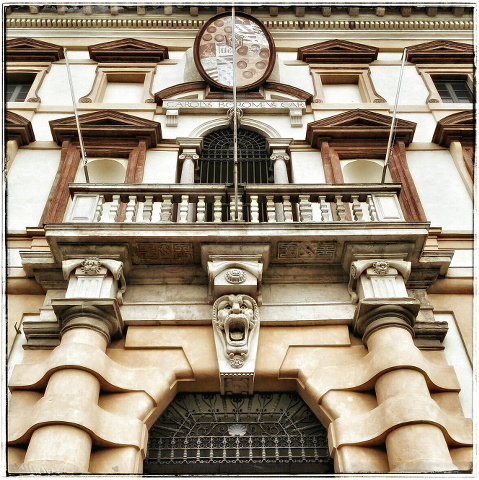
\includegraphics{smallthumb-lesson_I.jpeg}
\setfloatalignment{b}
\end{marginfigure}


\begin{abstract}
\noindent
Queste lezioni riprendono il testo introduttivo al Latino di Pearson\cite{pearson1915}, del quale seguono la numerazione; la struttura di ogni lezione è piuttosto regolare: inizia con \textsc{cenni di morfologia e di sintassi latina}, seguita da un \textsc{piccolo vocabolario} per il lessico; ci sono infine vari \textsc{esercizi} di traduzione e di composizione latina.

\bigskip
\noindent
Lezione XIII - Prima coniugazione (continua). Piucheperfetto e Futuro Perfetto. Ripasso, vocabolario, esercizi.
\end{abstract}

%\printclassoptions

% āēīōū
% ăĕĭŏŭ

\newthought{98. Prima Coniugazione, Piuccheperfetto.} Ripassa la sezione (81.)

\begin{fullwidth}
\begin{table}[!htbp]
  \centering
  \begin{tabular}{l l}
    %\toprule
	
	\multicolumn{2}{c}{\textsc{Indicativo Piuccheperfetto Attivo} di \textbf{amō}, \textit{io amo}} \\
	
	& \multicolumn{1}{c}{\textsc{Singolare}} \\

    \textsc{1.} & amāv\textbf{eram}, \textit{io avevo amato}   \\
    \textsc{2.} & amāv\textbf{eras}, \textit{tu avevi amato}  \\
    \textsc{3.} & amāv\textbf{erat}, \textit{egli aveva amato}   \\
   
	& \multicolumn{1}{c}{\textsc{Plurale}} \\
	
    \textsc{1.} & amāv\textbf{erāmus}, \textit{noi avevamo amato}    \\
    \textsc{2.} & amāv\textbf{erātis}, \textit{voi avevate amato}    \\
    \textsc{3.} & amāv\textbf{erant}, \textit{essi avevano amato}    \\
	
	\multicolumn{2}{c}{\textsc{Indicativo Futuro Perfetto Attivo}} \\
	
	& \multicolumn{1}{c}{\textsc{Singolare}} \\

    \textsc{1.} & amāv\textbf{erō}, \textit{io avrò amato}   \\
    \textsc{2.} & amāv\textbf{eris}, \textit{tu avrai amato}  \\
    \textsc{3.} & amāv\textbf{erit}, \textit{egli avrà amato}   \\
   
	& \multicolumn{1}{c}{\textsc{Plurale}} \\
	
    \textsc{1.} & amāv\textbf{erimus}, \textit{noi avremo amato}    \\
    \textsc{2.} & amāv\textbf{eritis}, \textit{voi avrete amato}    \\
    \textsc{3.} & amāv\textbf{erint}, \textit{essi avranno amato}    \\
	
    %\bottomrule
  \end{tabular}
  %\caption[bottom]{Prima Coniugazione, Piuccheperfetto e Futuro Perfetto.}
  \label{tab:normaltab}
  %\zsavepos{pos:normaltab}
\end{table}
\end{fullwidth}

\newthought{Osservazioni}
\begin{itemize}
\item[\textsc{1.}] Il piuccheperfetto è formato dalla combinazione del tema del perfetto \textbf{amāv-} e di \textbf{-eram};
il futuro perfetto (futuro anteriore) dalla combinazione dello stesso tema e di \textbf{-ero}. 
Vi è però un'eccezione in una forma del futuro perfetto, quale?
\end{itemize}

\newthought{99. Ripasso dell'Indicativo Attivo.} Ripassa con cura le sezioni (43.), (85.), (86.), (87.) e (92.).
Osserva come il \textit{tema del presente} venga usato nella formazione dei tempi presente, imperfetto e futuro, mentre
il \textit{tema del perfetto} venga usato nella formazione dei tempi perfetto, piuccheperfetto e futuro perfetto.

\begin{fullwidth}
\begin{table}[!htbp]
  \centering
  \begin{tabular}{l l}
    %\toprule
	
	\multicolumn{2}{c}{\textsc{Tabella per le forme verbali dell'Indicativo Attivo}} \\
	
    \textsc{Presente} & La prima parte principale del paradigma del verbo.   \\
    \textsc{Imperfetto} & Tema del presente + \textbf{bam}.   \\
    \textsc{Futuro} & Tema del presente + \textbf{bō}.   \\
   
   \textsc{Perfetto} & La seconda parte principale del paradigma del verbo.   \\
   \textsc{Piuccheperfetto} & Tema del perfetto + \textbf{eram}.   \\
   \textsc{Futuro Perfeto} & Tema del perfetto + \textbf{erō}.   \\
   
    %\bottomrule
  \end{tabular}
  %\caption[bottom]{Prima Coniugazione, Piuccheperfetto e Futuro Perfetto.}
  \label{tab:normaltab}
  %\zsavepos{pos:normaltab}
\end{table}
\end{fullwidth}

\newthought{100. Esercizio} Dire le parti principali, formare la prima persona singolare di tutti i tempi
del modo indicativo e tradurre i seguenti verbi (dai vocabolari precedenti):

\begin{multicols}{5}
    \noindent laudō  \\
    \noindent vocō  \\
	\noindent parō  \\
	\noindent oppugnō  \\
	\noindent servō  \\
	\noindent culpō  \\
	\noindent convocō  \\
	\noindent dō  \\
	\noindent portō  \\
	\noindent superō  \\
\end{multicols}

\begin{itemize}
\item[\textsc{1.}] Dire la coniugazione completa per tutti i tempi dell'indicativo di almeno tre verbi tra questi.  
\end{itemize}

% āēīōū
% ăĕĭŏŭ

\newthought{101. Vocabolario} 

\begin{multicols}{2}
	\noindent \hangindent=1em \textbf{maturō, -as, -āvī, -ātum, -āre}, v.tr. e intr., con l'infinito, \textit{far maturare, terminare, accellerare, anticipare, afrettarsi}.  \\
	\noindent \hangindent=1em \textbf{expugnō, -as, -āvī, -ātum, -āre}, v.tr., \textit{catturare, espugnare}.  \\
    \noindent \hangindent=1em \textbf{mox}, avv., \textit{subito, presto}.  \\	
	\noindent \hangindent=1em \textbf{ferus, a, um}, agg, \textit{selvaggio, barbaro}.  \\
	\noindent \hangindent=1em \textbf{impedimentum, -i}, n., \textit{ostacolo}, pl. \textit{bagagli}.  \\
    \noindent \hangindent=1em \textbf{vicus, -ī}, n., \textit{villaggio}.  \\
	\noindent \hangindent=1em \textbf{ad}, prep. con \acc, \textit{verso, a}.  \\
	
\end{multicols}
% āēīōū
% ăĕĭŏŭ

\newthought{102. Esercizi di Ripasso}
\\
\textsc{I.} \quad
\textsc{1.}~Gladiis et sagittis incolas oppidi superaverunt. \quad
\textsc{2.}~Contra Romanos bellum Galli parabunt. \quad
\textsc{3.}~In oppido Helvetiorum erit cibi inopia. \quad
\textsc{4.}~Legatus agricolas pilis armavit. \quad
\textsc{5.}~Gladium pulchrum Marco nautae perito dederunt. \quad
\textsc{6.}~In oppidum puellas et pueros convocabant.
\\
\textsc{II.} \quad
\textsc{1.}~Vi era abbondanza di grano nei campi del mio amico. \quad
\textsc{2.}~Le frecce, regalo della regina, piacquero al messaggero. \quad
\textsc{3.}~Non combatterà con le armi. \quad
\textsc{4.}~Hanno dato un bel cavallo alla donna. \quad
\textsc{4.}~Ha armato molti schiavi?



\newthought{103. Esercizi}
\\
\textsc{I.} \quad
\textsc{1.}~Maturaveras; laudaveris; expugnaverant. \quad
\textsc{2.}~Portaveritis; delectaveratis ; dederamus. \quad
\textsc{3.}~Arma comparare maturavit. \quad
\textsc{4.}~Parvum Helvetiorum oppidum expugnaverant. \quad
\textsc{5.}~Multa impedimenta in vicum portaverimus. \quad
\textsc{6.}~Dona ad reginam portabant. \quad
\textsc{7.}~Reginae copiae ferae erant. \quad
\textsc{8.}~Ad oppidum frumenti copia erat. \quad
\textsc{9.}~Incolas insulae tells armabimus. \quad
\textsc{10.}~Gladiis ad impedimenta pugnaverant. \quad
\textsc{11.}~Magnam pecuniam incolis non dedimus. \quad
\textsc{12.}~Mox in agris latis Gallorum erit frumentum. 
\\

\textsc{II.} \quad
\textsc{1.}~Egli si affretterà; si sarà afrettato. \quad
\textsc{2.}~Avevano dato, abbiamo dato; avrai lodato. \quad
\textsc{3.}~Aveva portato molto bagaglio in città. \quad
\textsc{4.}~Prenderanno subito molte città. \quad
\textsc{5.}~Perché non si affrettò a fornire del grano? \quad
\textsc{6.}~Vicino al bel villaggo vi erano ampi campi. 

\begin{figure}[!b]
  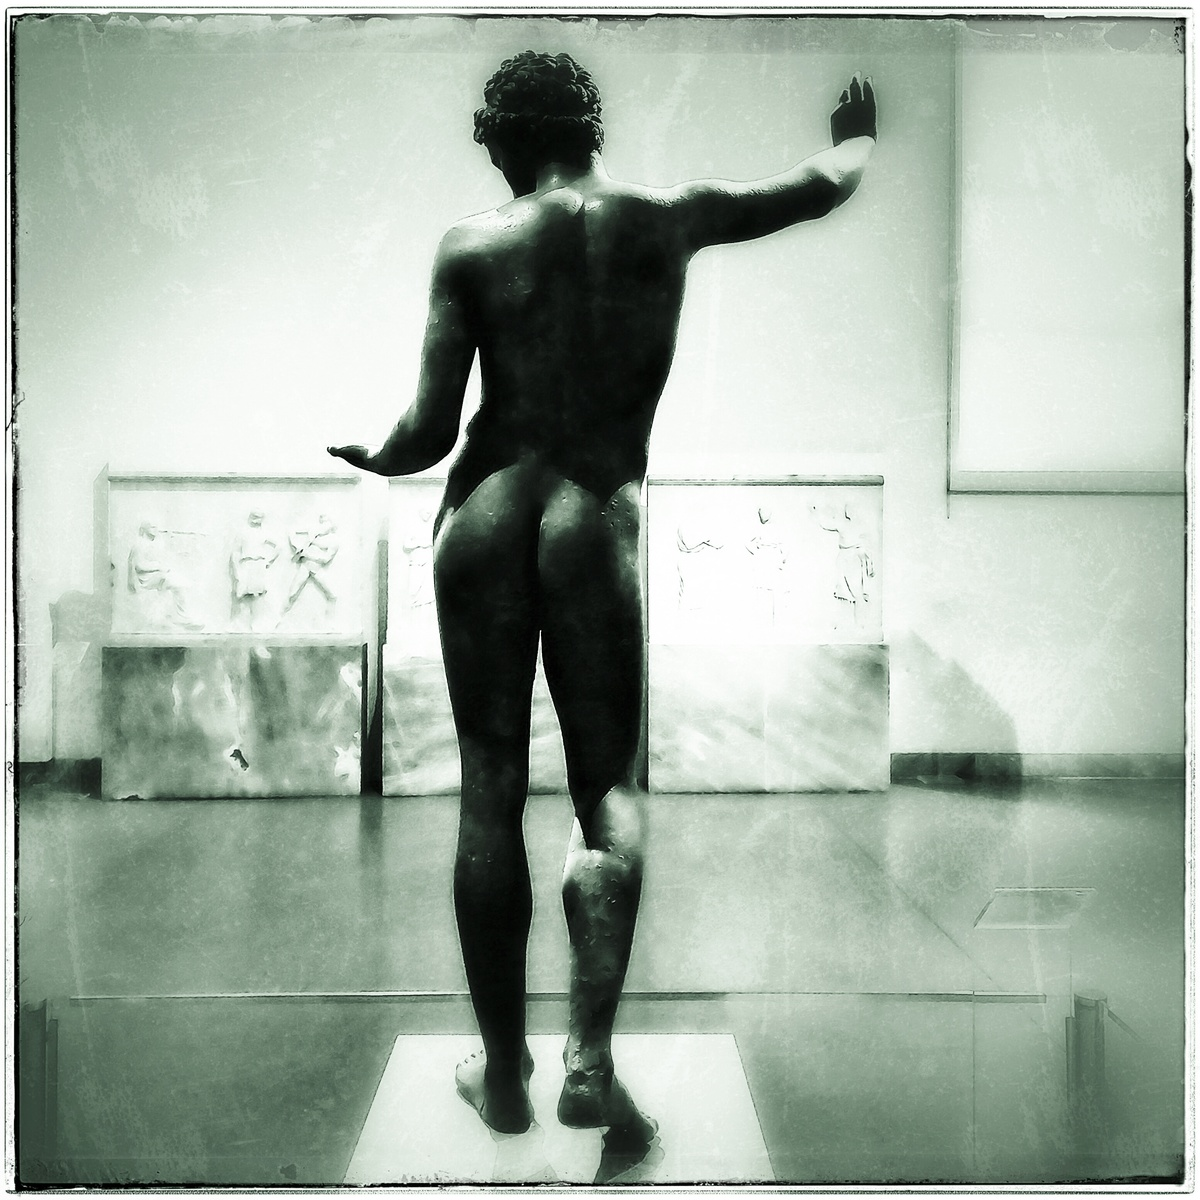
\includegraphics[width=0.8\linewidth]{thumb-lesson_VII.jpeg}
  %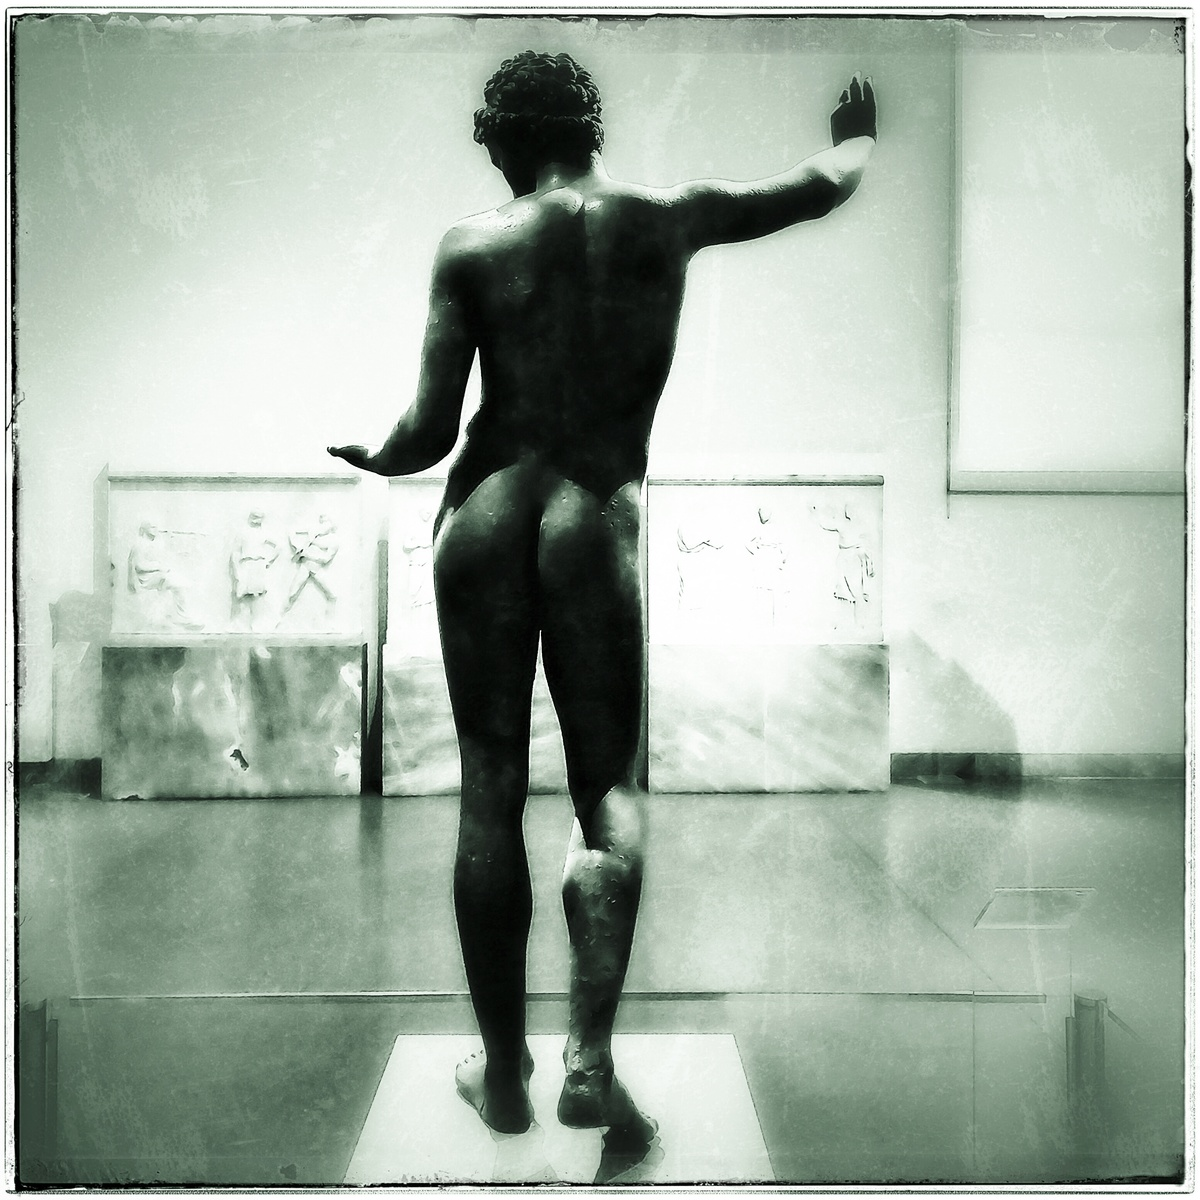
\includegraphics{thumb-lesson_VII.jpeg}
  \caption{Pavia: Almo Collegio Borromeo}
  \label{fig:textfig}
  %\zsavepos{pos:textfig}
  %\setfloatalignment{b}
\end{figure}

 

\nobibliography{latinBiblio}
\bibliographystyle{alpha}


\end{document}
